\documentclass[xcolor=dvipsnames,leqno]{beamer} 

\usetheme{Copenhagen}
%\beamersetuncovermixins{\opaqueness<1>{25}}{\opaqueness<2->{15}}
\beamertemplatenavigationsymbolsempty

\setbeamertemplate{frametitle}
{
\begin{flushleft}

\color{Blue}
\textbf{\large\insertframetitle}
\end{flushleft}
}

\setbeamertemplate{headline}
{%
  \leavevmode%
  \begin{beamercolorbox}[wd=.5\paperwidth,ht=2ex,dp=1.125ex]{section in head/foot}%
    \hbox to .5\paperwidth{\hfil\insertsectionhead\hfil}
  \end{beamercolorbox}%
  \begin{beamercolorbox}[wd=.5\paperwidth,ht=2ex,dp=1.125ex]{subsection in head/foot}%
    \hbox to .5\paperwidth{\hfil\insertsubsectionhead\hfil}
  \end{beamercolorbox}%
}
\expandafter\def\expandafter\insertshorttitle\expandafter{%
  \insertframenumber\,/\,\inserttotalframenumber} 
\insertsectionhead 
\insertsubsectionhead 

%\usepackage{xcolor}
\usepackage{hyperref}
\usepackage{textcomp}
\usepackage{setspace}
%\usepackage[options]{mcode}
%\usepackage{listings}
\usepackage{algorithmic} 
\usepackage{environ}
\usepackage {mathrsfs}
\NewEnviron{omitframe}{}
\usepackage{lmodern}   
\usepackage{bib entry}
\nobibliography*
\let\newblock\relax
\setbeamertemplate{navigation symbols}{}
\setbeamercolor{upcol}{fg=black,bg=Periwinkle}
\setbeamercolor{lowcol}{fg=black,bg=Periwinkle!40}

\newcommand*{\bigchi}{\mbox{\Large$\chi$}}
\newcommand{\R}{\mathbb{R}}
\renewcommand{\P}{\mathbb{P}}
\newcommand{\E}{\mathbb{E}}
%\newcommand{\C}{\mathbb{C}}
\newcommand{\N}{\mathbb{N}}

\newtheorem{algorithm}{Algorithm}
\newtheorem{thm}{Theorem}
\newtheorem{cor}[theorem]{Corollary}
\newtheorem{lem}[thm]{Lemma}
\newtheorem{prop}{Proposition}
\newtheorem{defn}{Definition}
\newtheorem{rmk}{Remark}
\newtheorem{eg}{Example}   

\title{Stochastic Navier-Stokes Equations perturbed by cylindrical L\'evy noise on 2D rotating sphere}

\author[Leanne Dong]{Leanne Dong\\
\vspace{1cm}{\small Supervised by: Prof. Ben Goldys}}
\vspace{1cm}
\institute[Usyd]{School of Mathematics and Statistics\\
University of Sydney}
%\titlegraphic{}
\date{November, 2016}
\setbeamersize{text margin left=0.5cm,text margin right=0.5cm}



\begin{document}
%\nobibliography*
	\begin{frame}
	  \titlepage
	\end{frame}

\section[]{Research rationales}  
\begin{frame}{Research rationales}
	\emph{Why study stochastic Navier-Stokes equations {\color{red}with noise, and {\color{red}stable} L\'evy noise}?}
	\begin{itemize}         
		\item More informative than deterministic equations.
		%\item The stochastic Navier-Stokes equations can model turbulence.
		\item To prove in a ``Cheaper" way for unsolved problems.\\
		\begin{itemize}
			\item Clay millenium problem No. 3: Uniqueness in 3D is missing.
			\item At atomic scale, fluid are not continuous fields
	%	\item Model complexity (especially turbulence, whether prediction) requires infinite dimensional analysis.
			\item L\'evy processes are perfect candidates to model discontinuity in infinite dimensions.
		\end{itemize}
	\end{itemize}
	\emph{Why stable-type L\'evy noise ?}
	\begin{itemize}
		\item Has a 'heavy tail' that decays polynomially. Useful for modelling extreme events - earthquakes, stock market crashes.
		\item Allows one to take into account at the same time noise with a large numer of small random impulses and occasionally large random disturbance with infinite moments.
	\end{itemize} 
\end{frame}

\begin{frame}
\frametitle{Research rationales: Rotating spheres?}
\begin{columns}
\column{0.5\textwidth}
\begin{itemize}
	\item Modelling large scale interactions between Ocean and atmosphere requires taking into account that we are on the surface of rotating Earth. 
	\item In cosmology, models of rotating fluids are used to describe many cosmological objects including black holes. (In this case, relativistic effects have to be taken into account which are not included in my thesis)
\end{itemize}
\column{0.5\textwidth}
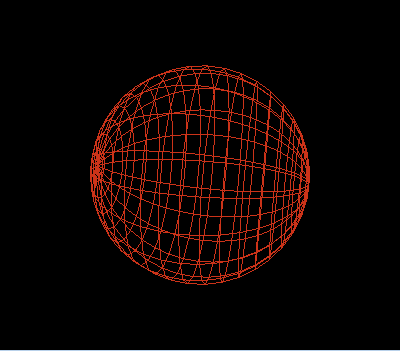
\includegraphics[scale=0.5]{Moving-Sphere.png}
\end{columns}
\end{frame}


\section{Problem formulation}
\begin{frame}[shrink]{The Navier-Stokes equations}
 We consider the stochastic Navier-stokes equations on the 2D unit sphere $\mathbb{S}^2\in (\theta,\phi)$ with rotation. Which is a system of 3 equations:
%\left\{
	\begin{align*}(1)
		\begin{cases}
			\partial_t u+ (u\cdot\nabla)u-\nu L u+\omega\times u+\nabla p=f+\eta(x,t) ,\quad\text{on} \,\, (t, x)\in (0, T)\times\mathbb{S}^2\\
			&\\
			\nabla\cdot u=0,\qquad\text{on} \quad (t, x)\in[0, T)\times\mathbb{S}^2, \quad{\color{RedOrange}\text{Incompressible condition}}\\
			&\\
			u(0)=u_0, \qquad\text{Initial conditions}	
		\end{cases}	
	\end{align*}  
%\right\}	        
\begin{itemize}
	\item $u, p, \nu, f$ are respectively velocity, pressure , viscosity and external forcing.
	\item $L=\Delta + 2\text{Ric}$ is the stress tensor, where $\Delta$ is the Laplace-de Rham operator and $\text{Ric}$ is the Ricci tensor on spheres.
	\item $\omega$ is the Coriolis acceleration which can be formally represented as $\omega(\cdot) = 2\Omega\cos\theta(\cdot)$.
	\item The noise process $\eta(x,t)$ can be viewed as some generalised derivative of $H$-valued L\'evy process.
\end{itemize}
\end{frame}

\begin{frame}
	The sphere can be viewed as a surface embedded into $\R^3$, hence, given any two vector fields $u$, $v$ on $\mathbb{S}^2$, we can find vector fields $\tilde{u}$ and $\tilde{v}$ defined on some nbhd of the surface $\mathbb{S}^2$ such that their restriction to $\mathbb{S}^2$ are equal to, resp. $u$ and $v$, namely,
	\begin{align*}
		\tilde{u}|_{\mathbb{S}^2}=u\in T\mathbb{S}^2\quad\text{and}\quad\tilde{v}|_{\mathbb{S}^2}=v\in T\mathbb{S}^2 
	\end{align*}
So, define orthogonal projection $\pi_x:\R^3\to T_x \mathbb{S}^2$

Then usual spherical calculus can be used to calculate standard curl and div operators.
\end{frame}

\begin{frame}{Weak formulation of Stochastic Navier Stokes Equations}
\begin{itemize}
	\item Orthogonal-projection $P_{\mathcal{L}} : H\to H_{\mathcal{L}}$
	%\item Let $\mathcal{P}$ be the Leray-Hopf operator. It is often written as
	 %it is a matrix valued Fourier multiplier given by
	\begin{align*}
		P_{\mathcal{L}}&=\text{Id}-\Delta^{-1}(\nabla\otimes\nabla).
	\end{align*}
	%It is an orthogonal projection of $(L^2(\mathscr{O}))^2$ onto $E$, which  
 $P_{\mathcal{L}}$	decomposes the velocity vector into its {\color{purple}divergence free part} and the {\color{orange}gradient of the scalar part}, that is, 
	\begin{align*}
		u={\color{purple}P_{\mathcal{L}}[(u\cdot\nabla)u]}+{\color{orange}\nabla \phi}
	\end{align*}
	\item Define $A: D(A)\to H$ by $Au=-\nu P_{\mathcal{L}} L u$, $D(A)=(H^2(\mathbb{S}^2))^2\cap V$.
	\item Define $B: V\times V\to V^{*}$ by $B(u,v)=P_{\mathcal{L}}[(u\cdot\nabla)v]$.
	\item $L(t)=P_{{\mathcal{L}}}\tilde{L}(t)$.%, $\tilde{L}(t)$ is a cylindrical L\'evy process takes value in $E$.    
	\item $B(u)=P_{\mathcal{L}}[\, \text{div}(u\otimes u)\, ]=P_{\mathcal{L}}[\text{div} \, uu^{T}]=B(u,u)$%\mathcal{P}[(u\cdot\nabla) u]$
\end{itemize}	
\end{frame}
\begin{frame}
Then, projecting (1) onto $H$ yields 
\begin{align*}
	\begin{cases}
	u_t=-\nu Au-B(v+z,v+z)-Cv+\alpha z+f,\,\,(t, x)\in (0, T)\times\mathbb{S}^2 \\
		u(0)=u_0\in H
	\end{cases}
\end{align*}
%leads to the abstract equations, which is the version of two-dimensional Stochastic Navier-Stokes equations in $u=u(t)=u(t,x)$ 
Suppose we have solved the projection problem (2) by finding the mild solution $u=P_{\mathcal{L}} u$, how do we recover the pressure from its projection?\\
\vspace{1cm}
\textbf{Answer}: By Hodge decomposition, the pressure satisfies

\[
	\nabla p=\nu\Delta u+(u\cdot\nabla)u-\partial_t \tilde{L}(t)-\mathcal{P}[-\nu\Delta u+(u\cdot\nabla)u-\partial_t \tilde{L}(t)]
\]
Solve for $u$, Substitute $u$ back to (1), we can recover $\nabla p$ in term of forcing term and the solution $u$.
\end{frame}
     
\begin{frame}{My problem}  
Projecting (1) onto $H$ leads to a version of the two-dimensional Navier-Stokes equation of our interest, which is the abstract equation in $u=u(t)=u(t,x)$:
	\begin{align*}\tag{2}%\label{iacp1e}
			\begin{cases}
		        du(t)+(Au(t)+B(u(t)))dt+Cu=fdt+GdL(t), \qquad t>0\\
				u(0)=u_0\in V%\,\,x\in\mathbb{R}
			\end{cases}
	\end{align*}  
%	has the mild form cylindrical solution of the form
We assume $A$ generate a strongly continuous semigroup $\{S(t): t\geq 0\}$ on $X$.  $\{u(t)\in X,t\geq 0\}$ is said to be a mild solution of (1) if
		\begin{align*}
			u(t)&=S(t)u_0-\hspace{-0.15cm}\int_{0}^{t} S(t-s)B(u(s))ds+\hspace{-0.15cm}\int_{0}^{t}[S(t-s)]GdL(s).\tag{3}
	%		&=S(t)u(0)-\int_{0}^{t}S(t-s)B(u(s)+L_{A}(s))ds\tag{4}
	%		&=S(t)u_0+F(u+L_A)(t)
		\end{align*}
%is satisfied for every $u(0)$.
%	{\color{red} Aim}: Well-posedness, regularity and ergodicity of the mild solution
\end{frame} 
\begin{frame}{Weak formulation of Stochastic Navier Stokes Equations}
	Define $z(t)=L_A(t)=\int_{0}^t S(t-s)GdL(s)$ as the solution of
	\begin{align*}
		\begin{cases}
			dz(t)+\hat{A}z(t)=dL(t), t\geq 0\\
			z(0)=0
		\end{cases}
	\end{align*}
With this definition, (3) can be written as
\begin{align*}
	u(t)=S(t)u(0)+\int_{0}^{t}S(t-s){\color{purple}B}(u(s)+z(s))ds
\end{align*}
\end{frame}              
    
        
\end{document}